\newpage


\section{Known host management}
\label{sec:knownHostManagement}

% Problem statement
Known host management in an unstructured peer-to-peer system is arguably simpler than in a structured peer-to-peer architecture. Graphically, if a node is a vertex, its known hosts determines its edges. The direction of the edges imply `who knows who', i.e., if nodes are known to each other, the edge is bidirectional. It is also possible that the hosts are not mutually known to each other.

In a structured network, a certain topology needs to be maintained in order for the overlay network to behave as intended\cite{stoica2003chord}. In an unstructured topology, there is no need to maintain known hosts in a specific structure, however, maintaining a balance between the amount of known hosts so that the network is sufficiently connected to function effectively, but not too many as to exceed a node's resources, is important\cite{lua2005survey}. Node's have finite memory to store known hosts so peer selection becomes important.

\begin{figure}[ht]
    \centering
    
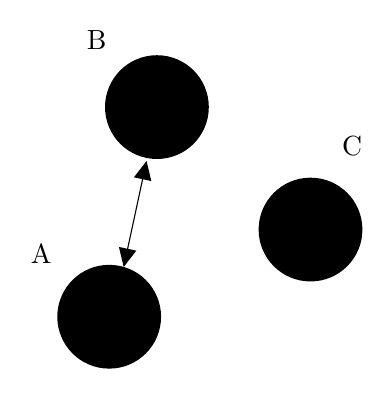
\begin{tikzpicture}[x=0.75pt,y=0.75pt,yscale=-1,xscale=1]
%uncomment if require: \path (0,300); %set diagram left start at 0, and has height of 300

%Shape: Circle [id:dp1418814839562289] 
\draw  [draw opacity=0][fill={rgb, 255:red, 0; green, 0; blue, 0 }  ,fill opacity=1 ] (116,196) .. controls (116,182.19) and (127.19,171) .. (141,171) .. controls (154.81,171) and (166,182.19) .. (166,196) .. controls (166,209.81) and (154.81,221) .. (141,221) .. controls (127.19,221) and (116,209.81) .. (116,196) -- cycle ;
%Shape: Circle [id:dp3981484481701938] 
\draw  [draw opacity=0][fill={rgb, 255:red, 0; green, 0; blue, 0 }  ,fill opacity=1 ] (139,95) .. controls (139,81.19) and (150.19,70) .. (164,70) .. controls (177.81,70) and (189,81.19) .. (189,95) .. controls (189,108.81) and (177.81,120) .. (164,120) .. controls (150.19,120) and (139,108.81) .. (139,95) -- cycle ;
%Shape: Circle [id:dp7390139799048381] 
\draw  [draw opacity=0][fill={rgb, 255:red, 0; green, 0; blue, 0 }  ,fill opacity=1 ] (213,154) .. controls (213,140.19) and (224.19,129) .. (238,129) .. controls (251.81,129) and (263,140.19) .. (263,154) .. controls (263,167.81) and (251.81,179) .. (238,179) .. controls (224.19,179) and (213,167.81) .. (213,154) -- cycle ;
%Straight Lines [id:da4506323249212101] 
\draw    (158.37,123.93) -- (148.63,169.07) ;
\draw [shift={(148,172)}, rotate = 282.17] [fill={rgb, 255:red, 0; green, 0; blue, 0 }  ][line width=0.08]  [draw opacity=0] (8.93,-4.29) -- (0,0) -- (8.93,4.29) -- cycle    ;
\draw [shift={(159,121)}, rotate = 102.17] [fill={rgb, 255:red, 0; green, 0; blue, 0 }  ][line width=0.08]  [draw opacity=0] (8.93,-4.29) -- (0,0) -- (8.93,4.29) -- cycle    ;

% Text Node
\draw (102,160) node [anchor=north west][inner sep=0.75pt]   [align=left] {A};
% Text Node
\draw (129,57) node [anchor=north west][inner sep=0.75pt]   [align=left] {B};
% Text Node
\draw (252,108) node [anchor=north west][inner sep=0.75pt]   [align=left] {C};


\end{tikzpicture}
    \caption{Three severely memory restricted nodes with no form of known host management}
    \label{fig:memoryRestrictedUnmanaged}
\end{figure}

\begin{figure}[ht]
    \centering
    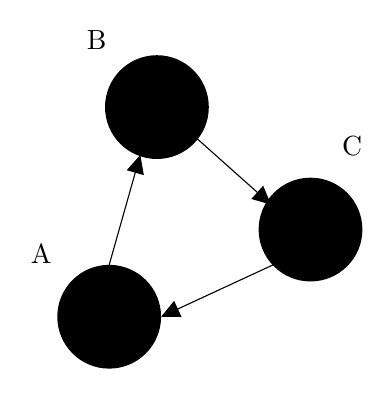
\begin{tikzpicture}[x=0.75pt,y=0.75pt,yscale=-1,xscale=1]
%uncomment if require: \path (0,300); %set diagram left start at 0, and has height of 300

%Shape: Circle [id:dp1418814839562289] 
\draw  [draw opacity=0][fill={rgb, 255:red, 0; green, 0; blue, 0 }  ,fill opacity=1 ] (116,196) .. controls (116,182.19) and (127.19,171) .. (141,171) .. controls (154.81,171) and (166,182.19) .. (166,196) .. controls (166,209.81) and (154.81,221) .. (141,221) .. controls (127.19,221) and (116,209.81) .. (116,196) -- cycle ;
%Shape: Circle [id:dp3981484481701938] 
\draw  [draw opacity=0][fill={rgb, 255:red, 0; green, 0; blue, 0 }  ,fill opacity=1 ] (139,95) .. controls (139,81.19) and (150.19,70) .. (164,70) .. controls (177.81,70) and (189,81.19) .. (189,95) .. controls (189,108.81) and (177.81,120) .. (164,120) .. controls (150.19,120) and (139,108.81) .. (139,95) -- cycle ;
%Shape: Circle [id:dp7390139799048381] 
\draw  [draw opacity=0][fill={rgb, 255:red, 0; green, 0; blue, 0 }  ,fill opacity=1 ] (213,154) .. controls (213,140.19) and (224.19,129) .. (238,129) .. controls (251.81,129) and (263,140.19) .. (263,154) .. controls (263,167.81) and (251.81,179) .. (238,179) .. controls (224.19,179) and (213,167.81) .. (213,154) -- cycle ;
%Straight Lines [id:da8506068290592598] 
\draw    (141,171) -- (155.18,120.89) ;
\draw [shift={(156,118)}, rotate = 105.8] [fill={rgb, 255:red, 0; green, 0; blue, 0 }  ][line width=0.08]  [draw opacity=0] (8.93,-4.29) -- (0,0) -- (8.93,4.29) -- cycle    ;
%Straight Lines [id:da3809501315965952] 
\draw    (182,109) -- (216.76,140) ;
\draw [shift={(219,142)}, rotate = 221.73] [fill={rgb, 255:red, 0; green, 0; blue, 0 }  ][line width=0.08]  [draw opacity=0] (8.93,-4.29) -- (0,0) -- (8.93,4.29) -- cycle    ;
%Straight Lines [id:da7416029981434609] 
\draw    (220,171) -- (168.72,194.74) ;
\draw [shift={(166,196)}, rotate = 335.16] [fill={rgb, 255:red, 0; green, 0; blue, 0 }  ][line width=0.08]  [draw opacity=0] (8.93,-4.29) -- (0,0) -- (8.93,4.29) -- cycle    ;

% Text Node
\draw (102,160) node [anchor=north west][inner sep=0.75pt]   [align=left] {A};
% Text Node
\draw (129,57) node [anchor=north west][inner sep=0.75pt]   [align=left] {B};
% Text Node
\draw (252,108) node [anchor=north west][inner sep=0.75pt]   [align=left] {C};


\end{tikzpicture}

    \caption{Three severely memory restricted nodes with known host management mechanism}
    \label{fig:memoryRestrictedManaged}
\end{figure}

One option is to simply choose known hosts on a `first-come-first-serve' basis, however, this causes issues in some cases. For example, take three severely memory restricted nodes that only have the capacity to store one known host each. Upon spawning, the first two would become aware of each other and hence store each other in their known host list, leaving the last node unknown and hence unable to participate in the network (illustrated in Figure~\ref{fig:memoryRestrictedUnmanaged}). This edge case highlights that we want to design a known host selection and maintenance protocol that, in addition to maintaining a list of alive known hosts, always accepts known hosts that would otherwise be unknown by the network (illustrated in Figure~\ref{fig:memoryRestrictedManaged}).

A few extra properties of known hosts might be desirable, for example, it might be easier to query large parts of the network if node $q$'s known hosts know a lot of other hosts. Furthermore, $q$ may want to have known hosts it can rely on, hence highly available. Finally, it might also be good to known hosts with lots of available storage so that $q$ can readily share information with its peers. Intuitively, we might be inclined to think that we should optimise known hosts to be highly available nodes, with plenty of available storage, that know lots of other nodes. However, if that were the case, new nodes would be actively disregarded by the network as they would inherently have low uptime and know relatively few other nodes. We have to make the distinction between what is good for the node and what is good for the network.

\subsection{Related work}

\subsubsection{Gnutella group membership messages}

While the Gnutella project does not implement a very complex known host management protocol it does implement a Group membership protocol in which a peer joining the network broadcasts $PING$ messages to announce its presence. The message is then forwarded to its neighbours, initiating back-propagated $PONG$ messages, which contain information about peers, such as the IP address, number and size of the data items.\cite{lua2005survey}

\subsubsection{JXTA peer information protocol}

Much like Gnutella, JXTA does not attempt to actively optimise a node's known hosts but provides a peer information protocol for peers to learn about the capabilities and status of others. For example, a $PING$ message can be sent to see if a peer is alive. A query can also be sent regarding a peer’s properties where each property is returned as a name and a value string.

\subsection{Design \& implementation}

In Butter, a node can query other remote nodes to obtain their $NodeQuality$ metadata. The data contained in $NodeQuality$ is: uptime, available storage space and number of known hosts. Nodes periodically request the $NodeQuality$ metrics from their known hosts and cache the data between updates.

% As an added optimisation, a node caches data when it updates its index of known host quality metric so as not to have to query its known hosts multiple times for many consecutive possible new host insertion

\subsubsection{Known host list maintenance}

Firstly, the simpler part of the Known host management module is handling dead known hosts. During the regular $NodeQuality$ requests, if a node is unresponsive, after a given timeout period, the host is removed from the list of known hosts. This reduces the probability that a node attempts to communicate with a dead host during other operations such as retrieving information or sharing discovered peers. Making sure that the hosts within the list are alive and responding with a minimum delay also prevents dead hosts from taking up list capacity, leaving room for new hosts to join.

\subsubsection{Peer selection}

In addition, the Known host management module is responsible for peer selection. Peer selection becomes a problem when a node's known host list is at capacity and hence decisions need to be made as whether knowing or ignoring a host is best (with regards to the node and the network).

The approach for designing peer selection is loosely inspired by various optimisation algorithms (optimal, sub-optimal and soft constraint). We define an optimisation problem to be: ``a set of variables, each with an associated domain, an objective function that maps total assignments to real numbers, and an optimality criterion, which is typically to find a total assignment that minimises or maximises the objective function"\cite{poole2017ai}. To avoid the edge case discussed previously, i.e., new peers being unable to get themselves known by pre-existing nodes on the network as they do not fit the desired $NodeQuality$, each node attempts to optimise its list of known hosts for a diverse distribution of $NodeQuality$s. In other words, nodes do not optimise for a specific kind of remote host but rather a diverse set of hosts. To put it in terms of an optimisation problem, the possible known hosts is the set of variables, each with an associated $NodeQuality$, the objective function determines how diverse the a known host list is (based on the node's own perception of diversity guided by its partial view) and the optimality criterion is to find a set of known host that maximises the node's known host diversity.\\

\noindent The procedure is as follow:
\begin{itemize}
    \item Trivially, if a node has sufficient memory to store a host, and does not already know it, store it (greedy philosophy)
    \item If the node is at capacity, determine, based on the characteristics of the node and those of its previously known hosts, whether the new host would make the list of known hosts more diverse
    \begin{itemize}
        \item If it does, remove a host from the most popular class of known host types and store the new one
        \item Else, do nothing
    \end{itemize}
\end{itemize}

Notice that this algorithm is somewhat reminiscent of the AI optimisation algorithms where given a current known host list state, we evaluate a permutations and consider whether the new states is an improvement or not.

The objective function for diversity is based on the node's partial view. A node looks at its metadata and the metadata of all of its immediate known hosts and classifies them according to this understanding of the network. With this objective function, at capacity, a node will attempt to have an equal distribution of node types, i.e., with varying $NodeQuality$ metrics, by mostly accepting nodes that increase the diversity of its list of known hosts.

% THIS IS VERY IMPORTANT - answers Nathan's question
An important edge case to consider is when many nodes are spawned in quick succession, with similar parameter settings, e.g., similar user allocated memory. This leads to many nodes with very similar $NodeQuality$ values. In this case, any given node will be optimising for a diverse set of known hosts, but the diversity between nodes and hence the global diversity may be poor. This results in the network converging towards knowing the same hosts. This can be thought of in terms of local and global diversity. % giving rise to the notion of internal (local) diversity and external (global) diversity.

In this scenario, all nodes have similar uptime, available storage and number known hosts, and hence have the same diversity metric. If a new node wants to joins the network, it runs through the Discovery protocol (as it knows no hosts) and is quickly accepted by a host (as hosts always accept nodes with no known hosts). However, if the node does not fit within the unanimous diversity metric it will quickly be rejected by the network, it will then go back into discovery mode, be discovered and eventually rejected once again. This will keep re-occurring.

A solution would be to not have any form of diversity driven optimisation and simply accept nodes at random, however, this may lead to uneven distribution of information on the network and poor network performance. Instead, we rely on a few factors to decrease the probability of this occurring. Firstly, in most practical environments nodes are not symmetric, nodes typically have their own very unique perception of the world as they have their own uptime, available storage (user allocated memory) and collection of known hosts. In addition a randomness factor is added to the diversity protocol. This means that on occasion a node is accepted or removed by chance despite its valuation by the objective function, i.e., regardless of the diversity metric. This prevents a convergence towards only accepting certain node types in an attempt to improve the probability of global diversity.

% In addition, It is worth noting that the probability of this edge case occurring in practice is somewhat mitigate by the fact that it is uncommon that many hosts all spawn at the same time (unless in simulated testing environments) and even more unlikely that nodes are symmetrical i.e. have exactly the same user specified allocated memory and hence the same amount of known hosts and available storage. By relying on the practical asymmetry between nodes and the added random acceptance we can mitigate the risk of a homogeneous global diversity. Known hosts are not symmetrical each is unique in the sense it has properties such as available memory, different uptime different set of known hosts - this means each node has a unique notion of what diverse based on its experience - this results in the overall network being diverse

\subsection{Testing \& evaluation}

% TODO: Get some hard numbers in for this somehow. e.g. in a a randomised network what is the diversity of peers? The NetworkX Python library might be a good fit

% \subsubsection{Known host list maintenance}

An extra optimisation to improve known host list maintenance would be to remove hosts that are found dead when carrying out other operations such as information retrieval. This would allow the list of known host to be updated between $NodeQuality$ request intervals. To achieve this we would have to introduce an API endpoint within the Known host management module to enable other modules to make changes to the known host list. However, this has the potential to increase complexity for developers and increases the risk of accidental mismanagement and incorrect removal of known hosts, so this feature is not implemented in the current version of the module.

During the implementation several different $NodeQuality$ intervals were explored. Obviously, short intervals means that the known host list is a better representation of the known hosts, however, this leads to greater message complexity. The message complexity of the $NodeQuality$ procedure grows linearly for a node based on the number of known hosts. On the other hand, the queries are exponential on a network level, as each node is querying its known hosts. The $NodeQuality$ interval should be a balance between maintaining an accurate reflection of the hosts and minimising network flooding.

% Maybe we should really be looking at Uptime or Storgae or Known host count and not the host class, as the classes are not comparable between nodes (each node has its own personal definition for a host type class.

\begin{table}[h]
    \centering
    \begin{tabular}{|l|c|c|c|}
        \hline
        \textbf{Test} & \textbf{S.D. Node A} & \textbf{S.D. Node B} & \textbf{Z-statistic} \\
        \hline
        No randomised acceptance, uniform nodes &  1.0897 & 0.9682 & 0.4797 \\
        Random acceptance, uniform nodes & 0.6614 & 0.9682 & 0.8472 \\
        Asymmetric nodes & 0.9990 &  0.8291 & 1.0640 \\
        \hline
    \end{tabular}
    \caption{Standard deviation of node types in three different test cases for two nodes chosen at random. Z-statistic is provided to compare distribution across the nodes.}
    \label{tab:diversityData}
\end{table}

% TODO: Remove the z stat because it is meaningless
In order to test the diversity mechanisms we generated several networks of Butter nodes at random using the testbed. The data from this experiment can be found in Table~\ref{tab:diversityData}. The standard deviation is a measure of distribution of host types. If the standard deviation is small, then we roughly have the same amount of each host type and the local diversity is relatively high. The $z$-statistic measure is used to compare the distribution between nodes.

% a low z-stat measure shows that the known hist list are similarly diverse across nodes

In the first instance of the test, nodes were spawned with the same allocated memory in quick succession, resulting in what we would assume to be similar host types. The mechanism that occasionally accepts a node at random regardless of host type was disabled. In this test, we observed slightly higher standard deviations of the host type distribution in comparisons to the other test environments. This suggests in a network with many uniform nodes, maintaining a diverse set of known hosts is more difficult. Note, that in all three testes, the difference in distribution of known hosts between the two nodes selected at random is fairly small suggesting there us little difference between the two distribution diversities. Once we introduce, the random acceptance mechanism, the standard deviation decreases suggesting there is greater diversity in the maintained list of known hosts.

In future it may be interesting to test how the network diversity mechanisms perform in prescribed topologies. Integrating the Butter testbed with tools such as NetworkX\cite{networkx2022networx, orda2019efficient} may allows the exploration of edge cases and provide a visual testing environment.

A last factor to consider is that $NodeQuality$ information becomes more quickly out-of-date on higher churn networks. If nodes are frequently dying and the interval is large, there is a higher probability that hosts in the list are unavailable. Currently the $NodeQuality$ update interval is a parameter that is user-specified. In a high-churn simulated environment (see Section~\ref{sec:churnTesting}) we saw significantly fewer failed requests when the update interval was 10 seconds as apposed to 30 seconds. An interesting future improvement might be to implement a dynamic update interval relying on some churn rate detection mechanism.

% \subsubsection{Peer selection}

% Another interesting parameter that can be changed is the frequency of accepting a new node at random and removing a node at random despite the objective function.

% Using the testing framework described in Section \ref{sec:testingMethodology} we compared the performance of information retrieval and persistent information storage on both unmanaged known hosts and managed known hosts. It was clear that 

Finally, in future, more metadata could be added to the $NodeQuality$ to broaden the diversity metric. For example, it may be interesting to give a sense of the information hosted by a peer, as having diverse knowledge between known hosts may increase the probability of quickly finding some piece of information.
